% ===============================================================================
% = LaTeX Beamer Template des Arbeitsbereichs Sicherheit in verteilten Systemem
% = (c) 2012 Prof. Dr. Hannes Federrath, Uni Hamburg, Fachbereich Informatik
% = http://www.informatik.uni-hamburg.de/svs/
% ===============================================================================
%
\documentclass[t, xcolor=dvipsnames]{beamer} 
% Option t              Place text of slides at the (vertical) top of the slides.
% Option handout        Ein PDF ohne Pausen und Overlayeffekte erzeugen.
% Option aspectratio=43 169 => 16:9, 1610 => 16:10, 43 => 4:3
\usepackage[utf8]{inputenc}
\usepackage[ngerman]{babel}
%\usepackage{graphicx}
\usepackage[T1]{fontenc} % 8-Bit-Zeichen; ermöglicht korrektes Kopieren von Umlauten aus dem pdf 
\usepackage[scaled]{helvet}

\usepackage{graphicx,xcolor}

\usepackage{beamerthemedefault}

\usepackage{tikz}
\usetikzlibrary{shapes,arrows}

% Ränder definieren
\setbeamersize{text margin left=5ex, text margin right=5ex}

% Farbdefinitionen
\definecolor{svsgrau1}{RGB}{191,191,191} % Balken in Kopfzeile
\definecolor{svsgrau2}{RGB}{123,123,123} % Folienüberschriften
\definecolor{svsrot}{RGB}{255,0,0} % Bullets
\definecolor{svshellblau1}{RGB}{153,204,255} % Block Hintergrund
\definecolor{svshellblau2}{RGB}{24,113,248} % Anstrich Ebene 2
\definecolor{svsdunkelblau}{RGB}{38,82,128} % Text der Ebene 1

% Navigationsleiste ausblenden
\beamertemplatenavigationsymbolsempty 

% Farben der Bullets der Ebenen
\setbeamercolor{itemize item}{fg=svsrot}
\setbeamercolor{itemize subitem}{fg=svshellblau2}
\setbeamercolor{enumerate item}{parent=itemize item}
\setbeamercolor{enumerate subitem}{parent=itemize subitem}

% Formen der Bullets der Ebenen
\setbeamertemplate{itemize item}[circle] 
\setbeamertemplate{itemize subitem}{--} 
\setbeamertemplate{itemize subsubitem}[circle] 

% Farben der Texte 
\setbeamercolor{title}{fg=black}
\setbeamercolor{structure}{fg=svsgrau2}
\setbeamercolor{section in toc}{fg=black}
\setbeamercolor{framesubtitle}{fg=svsdunkelblau}
\setbeamercolor{itemize/enumerate body}{fg=svsdunkelblau}
\setbeamercolor{itemize/enumerate subbody}{fg=black}
\setbeamercolor{itemize/enumerate subsubbody}{fg=black}

% Zeichensätze der Texte
\setbeamerfont{author}{size=\normalsize}
\setbeamerfont{institute}{size=\normalsize}
\setbeamerfont{date}{size=\normalsize}
\setbeamerfont{frametitle}{size=\large}
\setbeamerfont{framesubtitle}{size=\footnotesize\raggedleft}
\setbeamerfont{sections/subsections in toc}{size=\normalsize}
\setbeamerfont{itemize/enumerate body}{size=\normalsize}
\setbeamerfont{itemize/enumerate subbody}{size=\normalsize}
\setbeamerfont{itemize/enumerate subsubbody}{size=\normalsize}

% Definitionen für farbig hinterlegten Block 
\setbeamertemplate{blocks}[rounded]
\setbeamercolor{block title}{fg=black,bg=svshellblau1}
\setbeamercolor{block body}{parent=normal text,use=block title,bg=block title.bg!25!bg}
\setbeamerfont{block title}{size=\normalsize}
\setbeamerfont{block body}{size=\normalsize}

% Definitionen für Agenda (FIXME: noch stärker an normale Listendefs. anpassen)
\setbeamertemplate{section in toc}[sections numbered]
\setbeamertemplate{subsection in toc}[square]

% Kopfzeile
\setbeamertemplate{headline}{
	
\includegraphics[height=8mm]{pic/UHH-Logo_2010_ohneText.png}%
	\color{svsgrau1}\rule{\paperwidth}{8mm}\newline
	\mbox{}\rule{1em}{0pt}\rule{0pt}{8ex}
	\dotfill\newline\vspace{-7.3ex}
}

% Fusszeile
\setbeamertemplate{footline}[text line]{
	\parbox[b]{50mm}{\insertframenumber\\[1ex]}
}

% Hintergrund Titelseite
\defbeamertemplate{background canvas}{titlepage}{%
	{\color{svsgrau1}\vrule width\paperwidth height0.7\paperheight}%
	{\color{white}\vrule width\paperwidth height0.3\paperheight}%
}

% =============================
% = Ab hier Inhalte ändern... 
% =============================

\title{Das c-mix Verfahren }
\author[Merlin Koglin, Maik Graaf]{Merlin Koglin, Maik Graaf}
% \institute[Uni Hamburg]{Universität Hamburg\\ Fachbereich Informatik}
\date{}

\begin{document}

\begingroup
	\setbeamertemplate{background canvas}[titlepage]
	\begin{frame}[plain]
		\vskip8mm
		
\includegraphics[width=2.2cm]{pic/svs_logo_uhhred.png}
		% \vskip-20mm % dies geht nur bei kurzen Vortragstiteln
		\titlepage
		\vspace{\fill}
		
\includegraphics[width=2.9cm]{pic/UHH-Logo_2010_Farbe_RGB_hires_nomargin.png}
		\vskip20pt
	\end{frame}
\endgroup

\begin{frame}{Agenda}
	\tableofcontents
\end{frame}

\section{Motivation} % erscheint in Agenda


\begin{frame}
	\frametitle{Ansatz der Chaumische Mixe}
	\begin{itemize}
		\item Gewährleistung der Anonymität
			\begin{itemize}
				\item Mixe werden durchlaufen um die Beziehung zwischen Sender und Empfänger zu verschleiern
		        \item Im Mixnetz findet eine „Zwiebelschalen“ artige Entschlüsselung statt
		        \item Mithilfe der Rückadresse wird der Empfänger einer Nachricht bestimmt
			\end{itemize}
	\end{itemize}
	\vspace{\fill}
\end{frame}

\begin{frame}
	\frametitle{Probleme bisheriger Mix Verfahren}
	\begin{itemize}
		\item In Echtzeitsystemen
			\begin{itemize}
				\item Lange warte Zeiten beim Sammeln der Nachrichten
				\item Der Sammelschritt wird deshalb kurz gehalten oder sogar weggelassen
				\item Das Verfahren wird somit angreifbarer
				\item Für mobile Geräte ungeeignet aufgrund des großen Zeit und Energie Aufwands
			\end{itemize}
	\end{itemize}
	\vspace{\fill}
\end{frame}

\begin{frame}
	\frametitle{Idee von David Chaum}
	\begin{itemize}
		\item Vermeidung von Schlüsselberechnungen in Echtzeit 
			\begin{itemize}
				\item Steigerung der Effizienz von Mix-Netzen
				\item Energieaufwand verringern
				\item Schlüsselberechnung vor der Kommunikation
				\item Schlüssel Austausch zwischen Sender und Mixknoten
			\end{itemize}
	\end{itemize}
	\vspace{\fill}
\end{frame}

\section{Elgamal-Verschlüsselungsverfahren}
\begin{frame}
	\frametitle{Elgamal}
	\begin{itemize}
		\item Elgamal-Verschlüsselungsverfahren
			\begin{itemize}
				\item asymmetrisch
				\item basiert auf Diffie-Hellman-Schlüsselaustausch
				\item diskreter Logarithmus als Einweg-Funktion
				\item diskrete Exponentialfunktion $b^x \mod m$ -> einfach zu berechnen
				\item bisher kein effiziente Berechnung der Umkehrfunktion bekannt
			\end{itemize}
	\end{itemize}
	\vspace{\fill}
\end{frame}

\section{c-mix Verfahren} % erscheint in Agenda

\begin{frame}
	\frametitle{Kommunkationsübersicht}
	\begin{center}
				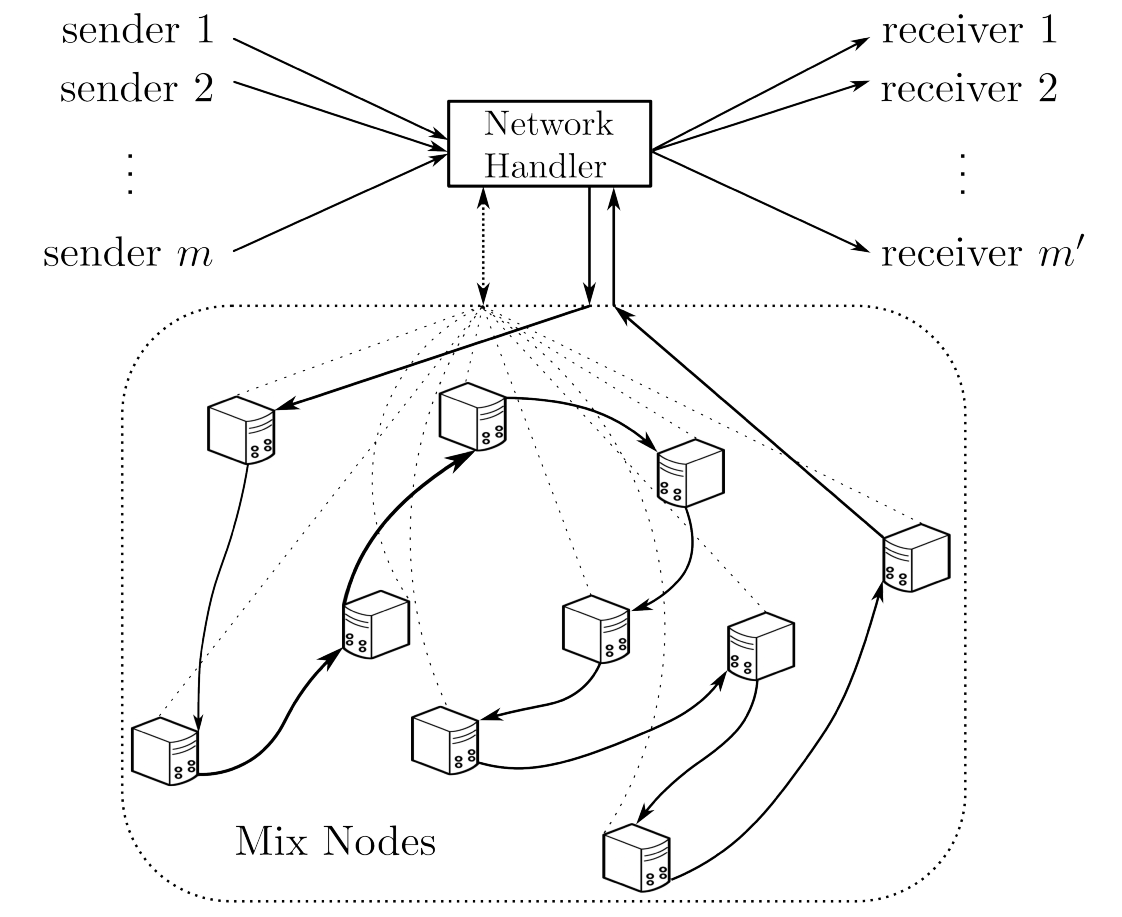
\includegraphics [width=0.8\textwidth]{pic/commover.png}
			\end{center}
	\vspace{\fill}
\end{frame}




\begin{frame}
	\frametitle{Übersicht der zwei Phasen}
	\begin{itemize}
		\item Precomputation Phase
			\begin{itemize}
				\item 1
			\end{itemize}
		\item Realtime Phase
			\begin{itemize}
				\item 2
			\end{itemize}
	\end{itemize}
	\vspace{\fill}
\end{frame}


\begin{frame}
	\frametitle{Vorbereitung}
	\begin{itemize}
		\item User
			\begin{itemize}
				\item Symmetrischer Schlüssel $K_{i,j}$ zwischen jedem User $U_j$ user jedem Node $N_i$ 
				\item Austausch des Schlüssels z.B. mit Diffie-Hellman
				\item $K_{i,j}$ wird später als Eingabe für Pseudozufallszahlengenerators verwendet
				\item User und Node könne für jede Runde den gleichen Schlüssel generieren.
			\end{itemize}
	\end{itemize}
	\vspace{\fill}
\end{frame}


\begin{frame}
	\frametitle{Precomputation - Step 1}
	\begin{itemize}
				\item Pre Processing

				\item Knoten $N_1$, ... $N_n$ erzeugt einen Vektor $r_i$ aus zufälligen Werten für jede Nachricht

				\item Verschlüsselung mittes ElGamal $\rightarrow$ $E(r_i^{-1})$, Resultat wird an den Network Handler gesendet
				\begin{itemize}
					\item Diese Verschlüsselung muss dann in der Echzeitphase nicht mehr durchgeführt werden
				\end{itemize}
				\item NH berechnet Produkt aus allen $E(r_n)$ $\rightarrow$ $E(R_n^{-1})$  
		\end{itemize}
	\vspace{\fill}
\end{frame}

\begin{frame}
	\frametitle{Precomputation - Step 2}
	\begin{itemize}
				\item Mixing
				\begin{enumerate}
					\item Jeder Knoten legt Permutation $P(X)$ fest.
					\item Jeder Knoten erzeugt einen weiteren zufälligen Vektor $s_i$
					\item $E(R_n^{-1})$ wird von jedem Knoten nacheinander mit der jeweils festgelegten Permutation permutiert (Mixing) und gleichzeit der erzeugte $s_i^{-1}$ hineinmultipliziert
					\item $s_i$ wird später für eine Nachrichtenantwort verwendet
				\item Der letzte Knoten erzeugt damit $E(P_n(R_n^{-1}) \times S_n^{-1})$
				\end{enumerate}

	\end{itemize}
	\vspace{\fill}
\end{frame}

\begin{frame}
	\frametitle{Precomputation - Step 3}
	\begin{itemize}
		\item Post Processing
		\begin{enumerate}
			\item Jeder Knoten berechnet nun aus $E(P_n(R_n^{-1}) \times S_n^{-1})$ seinen Entschlüsselungsanteil $D(i, r)$ für den zufälligen Vektor $r_i$ aus Schritt 1.
			\item Das jeder Knoten einen eigenen Entschlüsselungsanteil berechnen kann, liegt an der ElGamal Verschlüsselung, die diese Möglichkeit bietet.
			\item $E(P_n(R_n^{-1}) \times S_n^{-1})$ kann nur mit allen Anteilen entschlüsselt werden
		\end{enumerate}
		
	
	\end{itemize}
	\vspace{\fill}
\end{frame}

\begin{frame}
	\frametitle{Precomputation - Return Path}
	\begin{itemize}
		
		\item Step 1
		\begin{enumerate}
			\item Nodes erzeugen zufällige Vektoren $E({s'}_i^{-1})$ (ElGamal verschlüsselt).
			\item Permutation rückwärts, der letzte Knoten beginnt, gleichzeitig werden $s'^{-1}$ dazumultipliziert
			\item Der erste Knoten erhält $E({S'}_1^{-1})$
		\end{enumerate}
		\item Step 2
		\begin{enumerate}
			\item Wie vorher werden wieder Entschüsselungsanteile für $E({S'}_1^{-1})$ von allen Knoten berechnet
		\end{enumerate}
		\item 
		
		 
	\end{itemize}
	\vspace{\fill}
\end{frame}

\begin{frame}
	\frametitle{Precomputation - Resultat}
	\begin{itemize}
		
		\item Hinweg
		\begin{enumerate}
			\item $E(P_n(R_n^{-1}) \times S_n^{-1})$
		\end{enumerate}
		\item Rückweg
		\begin{enumerate}
			\item $E({S'}_1^{-1})$
		\end{enumerate}
		\item 
		
		 
	\end{itemize}
	\vspace{\fill}
\end{frame}


\begin{frame}
	\frametitle{Echzeit Phase - Step 1}
	\begin{itemize}
		\item Generierung mit gleichem Seed
		\begin{enumerate}
		\item User $U_j$ generiert aus $K_{i,j}$ Zufallszahl $ka_{i,j}$ für jeden Knoten, $Ka_j = \sum_{i=1}^n ka_{i,j}$
		\item Verschlüsselung einer Nachricht mit $\color{OliveGreen} M_j \times Ka_j ^{-1}$
		\item Network Handler $\color{OliveGreen}Ka_j ^{-1} \rightarrow Ka^{-1}$ $\rightarrow$ $\color{Mahogany} M \times Ka^{-1}$
		\item Knoten $N_i$ generiert $ka_i$ $= \sum_{j=1}^m ka_{i,j}$ und sendet $\color{BlueViolet}ka_i \times r_i$ an den NH.
		
		\end{enumerate}
		\item Austausch der Verschlüsselung
		\begin{enumerate}
		
		\item Der NH kann damit die $Ka^{-1}$ mit den zufälligen Vektoren $r_i$ der Knoten austauschen
		\item $ \color{Mahogany} M \times Ka^{-1}$ $\times \sum_{i=1}^n \color{BlueViolet}ka_i \times r_i$ $= M \times R_n$

		\end{enumerate}

		
	\end{itemize}
	\vspace{\fill}
\end{frame}

\begin{frame}
	\frametitle{Echzeit Phase - Step 2}
	\begin{itemize}
		\item Mixing
		\begin{itemize}
			\item Jeder Knoten permutiert (Nachrichten werden getauscht) nacheinander $M \times R_n$ und multipliziert den zufälligen Vektor $S_i$ mit ein
			\item Der letzte Knoten erhält damit $\color{Mahogany}P_n(M \times R_n) \times S_n)$
		\end{itemize}
	\end{itemize}
	\vspace{\fill}
\end{frame}

\begin{frame}
	\frametitle{Echzeit Phase - Step 3}
	\begin{itemize}
		\item Sammeln der Entschlüsselungsanteile
			\begin{itemize}
				\item Die Knoten $N_1$ bis $N_{i}$ senden ihren Entschlüsselungsanteil $D(i,x)$ an den NH
			\end{itemize}

		\item Entschlüsselung
		\begin{itemize}
				\item Der NH Entschlüsselt $\color{OliveGreen} E(P_n(R_n^{-1}) \times S_n^{-1})$ mittels $D(n,x)$
				\item $\color{Mahogany}P_n(M \times R_n) \times S_n$ $\times$ $\color{OliveGreen}P_n(R_n^{-1}) \times S_n^{-1} = \color{Emerald} P_n(M)$
		\end{itemize}

	
	
		\item Resultat
		\begin{itemize}
			\item $\color{Emerald} P_n(M)$ Ursprüngliche Nachrichten in vertauschter Reihenfolge
			\item Keine direkte Verbindung zum Sender möglich
		\end{itemize}
	\end{itemize}		
	\vspace{\fill}
\end{frame}


\begin{frame}
	\frametitle{Echzeit Phase - Antwort}
	\begin{itemize}
		\item Sammeln der Entschlüsselungsanteile
			\begin{itemize}
				\item Die Knoten $N_1$ bis $N_{i}$ senden ihren Entschlüsselungsanteil $D(i,x)$ an den NH
			\end{itemize}
		\end{itemize}
			
	\vspace{\fill}
\end{frame}


\section{Sicherheit}

\begin{frame}
	\frametitle{Anonymität}
	\begin{itemize}
		\item Anhand eines Modells
			\begin{itemize}
				\item Private Kommunikation der Mixknoten untereinander und eines vertraulichen dritten Punktes
				\item Keine Kryptographischen Operation, Sicherstellung durch den vertraulichen dritten Punkt
				\item „reale Simulation“ des Modells mit Eigenschaften des cMix Protokolls zeigt Anonymität
			\end{itemize}
	\end{itemize}
	\vspace{\fill}
\end{frame}

\begin{frame}
	\frametitle{Integrität}
	\begin{itemize}
		\item Die Integrität ist gegeben wenn
			\begin{itemize}
				\item Die Nachricht M unmodifiziert und an den Empfänger weitergeleitet wird oder...
				\item Alle Mixknoten wissen, dass das cMix Protokoll nicht richtig durchgeführt wurde
					\begin{itemize}
						\item Sicherstellung durch den Mechanismus „Randomized Partial Checking“
					\end{itemize}
			\end{itemize}
	\end{itemize}
	\vspace{\fill}
\end{frame}

\begin{frame}
	\frametitle{Vertraulichkeit}
	\begin{itemize}
		\item Schutzziel Anonymität
			\begin{itemize}
				\item Wird sichergestellt indem Nachrichten vom Sender verschlüsselt werden
					\begin{itemize}
						\item z.B durch einen öffentlichen Schlüssel einer asymmetrischen Verschlüsselung
					\end{itemize}
				\item Diese Verschlüsselung vermeidet aufwändige Publickey-Operationen 
			\end{itemize}
	\end{itemize}
	\vspace{\fill}
\end{frame}

\section{Performance}
\begin{frame}
	\frametitle{Protoyp}
	\begin{itemize}
		\item Performance Messung
			\begin{itemize}
				\item In Python implementiert
				\item Auf Instanzen des Amazon Web Service EC2 getestet
				\item Jeder Mixknoten hatte zwei Intel Xeon E5-2680 und 3,75 GB Arbeitsspeicher zur Verfügung
				\item Bei einer 1024-bit ElGamal-Verschlüsselung
				\item Starke Verbesserung das re-encryption Mixnet ist bis zu 8 mal	langsamer
			\end{itemize}
			
	\end{itemize}
	\begin{center}
				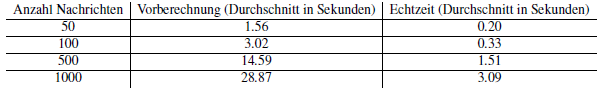
\includegraphics [width=1\textwidth]{pic/PrototypMessung.png}
			\end{center}
	\vspace{\fill}
\end{frame}

\section{PrivaTegrity}

\begin{frame}
	\frametitle{Einbettung in PrivaTegrity}
	\begin{itemize}
		\item Zweck
			\begin{itemize}
				\item Nur mit \alert{berechtigten Partnern} weiter kommunizieren
				\item Verhindert unbefugte Inanspruchnahme von Betriebsmitteln
			\end{itemize}
	\end{itemize}
	\vspace{\fill}
\end{frame}


\begin{frame}
	\frametitle{Backdoor}
	\begin{itemize}
		\item Zweck
			\begin{itemize}
				\item Nur mit \alert{berechtigten Partnern} weiter kommunizieren
				\item Verhindert unbefugte Inanspruchnahme von Betriebsmitteln
			\end{itemize}
	\end{itemize}
	\vspace{\fill}
\end{frame}

\end{document}
